\section{Statistische Modellierung}
Wir wollen uns noch einmal der Klassifikation zuwenden. Wie bereits
gesehen, sind Wahrscheinlichkeiten als Ergebnis einer Klassifikation
sinnvoller, als absolute Zuweisungen. Dafür gibt es nun im Folgenden
zwei Ansätze: \textbf{Naive Bayes} geht von der Unabhängigkeit
der Attribute aus (was selten der Realität entspricht, deswegen "'Naive"')
und \textbf{Bayesian Networks}, die die Korreliertheit der Attribute
berücksichtigen können.

\subsection{Naive Bayes}
\textbf{Standardfall:} Wir haben einen vollständigen Datenbestand 
mit seinen Klassenzugehörigkeiten. Wir bestimmen zunächst durch
Abzählen die relative Häufigkeiten der Klassenzugehörigkeiten, also
\(P[Klasse]\), und dann bestimmten wir die relativen Häufigkeiten
der Attributwerte pro Klasse, also \(P[x \mid Klasse]\). Dabei wird
\(P[Klasse]\) auch als \textit{Baysian Prior} bezeichnet. Ist dieser
nicht bestimmbar, so gehen wir einfach von einer Gleichverteilung der
Klassen aus.

Wenn wir nun die Klassenzugehörigkeitswahrscheinlichkeiten
eines neuen Objekte \(o\)
bestimmen wollen, lassen sich diese einfach durch
\[ P[Klasse \mid o] = \frac{\prod_j P[o_j \mid Klasse] \cdot P[Klasse]}{P[o]}\]
berechnen. \(P[o]\) fällt hier wieder weg, da man durch Normalisierung
sowieso \(P[o] = \sum_i P[o \mid Klasse_i] \cdot P[Klasse_i]\) berechnen
lässt. Des Weiteren gilt, dass sich \(P[o \mid Klasse]\) aufgrund
der Unabhängigkeitsannahme auch als Produkt der bedingten
Wahrscheinlichkeiten der einzelnen Attribute berechnen lässt. Daher das
Produkt über \(j\).

\textbf{Spezialfälle:} Auch hier kann das Fehlen von bestimmten
Attributwertkombinationen zu Problemen bei unseren Berechnungen führen.
Deswegen wird in solchen Fällen der Laplace Estimator verwendet. Dies
wird sich auf die Wahrscheinlichkeitsberechnung wie folgt aus:
Aus \([0, 5/10, 5/10]\) wird \([1/13, 6/13, 6/13]\). Man kann statt der
1 auch eine kleine Konstante addieren.

Ein anderer Fall wäre, dass im neu zu klassifizierenden Objekt
ein oder mehrere Attributwerte fehlen. Dies kann einfach behoben werden,
indem bei der Wahrscheinlichkeitsberechnung einfach die entsprechenden 
Faktoren ausgelassen werden.

Haben wir zum Teil auch numerische Werte, dann können wir nicht
mit relativen Häufigkeiten arbeiten. Für diese Attribute werden dann
Klassenweise Verteilungen angenommen und die Parameter für diese
berechnet (üblicherweise einfach die Normalverteilung annehmen).
Dann kann mit der Wahrscheinlichkeitsdichtefunktion wieder wie oben
die Klassenzugehörigkeitswahrscheinlichkeiten berechnen.

\subsection{Bayesian Networks}
Mit diesen Netzwerken können auch Korrelationen der Attribute
modelliert werden. Die Struktur des Netzwerks ist ein DAG (Directed Acyclic
Graph), der jeweils pro Attribut und pro Klasse einen Knoten besitzt.
Zwischen den Knoten gibt es genau dann eine Kante, wenn es eine Abhängigkeit
zwischen den beiden Knoteninhalten gibt. Zwischen Klassen-Knoten und
Attribut-Knoten gibt es \textbf{immer} eine Abhängigkeit. Die Richtung
der Abhängigkeit soll seine Kausalität modellieren; sie bestimmt lediglich
die Struktur der Wahrscheinlichkeitstabellen, die später in den Knoten
stehen werden. Damit sind durchaus auch unterschiedliche Darstellungen
des selben Sachverhaltes möglich.

Aus Gründen der Darstellbarkeit verzichten wir im Folgenden auf
Sonderfälle, wie fehlende Daten oder numerische Werte.

\begin{figure}[htbp]
	\centering
	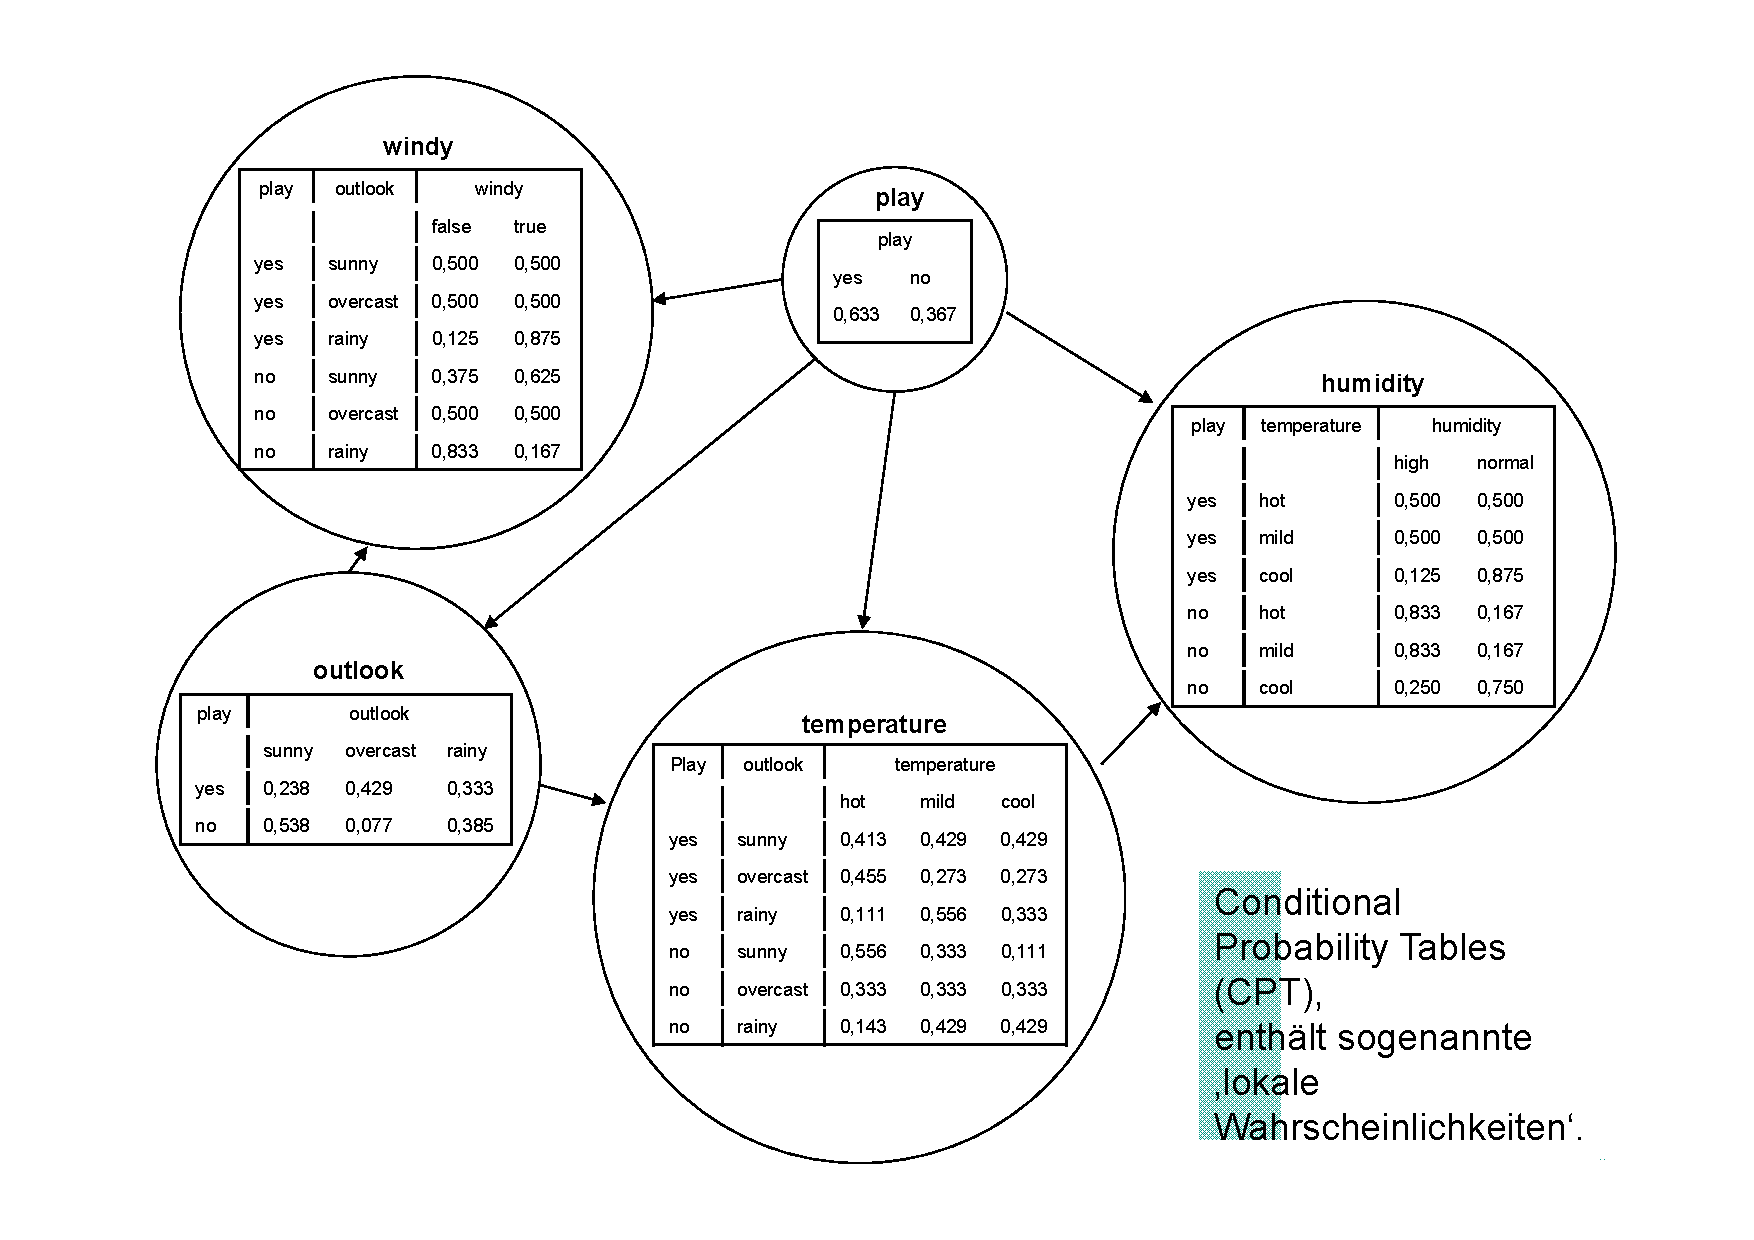
\includegraphics[width=0.75\textwidth]{Figures/cpt}
	\caption[BN Beispiel]{Beispiel für ein Bayesian Network.\footnotemark}
	\label{fig:cpt}
\end{figure}
\footnotetext{11. Foliensatz, S.33, Analysetechniken für große Datenbestände, Prof. Dr.-Ing. Klemens Böhm}

In Abb.~\ref{fig:cpt} ist ein Beispiel eines solchen Netzwerkes zu sehen.
Wie man sieht, wirken sich die Pfeile auf die Tabellen aus: In den
Tabellen stehen nun die von den abhängigen Attribute bedingten 
Wahrscheinlichkeiten. Man hat sieht, dass der Preis, den man für
die höhere Genauigkeit zahlt, die größere Zahl an Parametern ist.
Aber immerhin: Würde man explizit alle möglichen Attributwert-
Kombinationen in einer einzigen großen Zustandstabelle modellieren,
so hätte diese die Größe des Produkts der Anzahl an Attributen je
Attribut.

Neue Objekte lassen sich nun einfach Klassifizieren, indem man die
entsprechenden Wahrscheinlichkeiten für die Attribute aus dem Netzwerk
abliest und miteinander multipliziert. Die Grundannahme hierbei ist 
die so genannte \textbf{conditional independence}, nach welcher die
Werte von Attributen nur durch ihre Eltern-Attribute beeinflusst werden,
d.h. dass alle anderen Attribute maximal indirekt Einfluss nehmen können,
über die Eltern-Attribute. Semi-formal ergibt sich
\[
P[node \mid parents\ and\ any\ other\ nondescendants] = P[node \mid parents].
\]
Die Berechnung der neuen Vorhersage ergibt sich aus
\[
P[x_1,x_2,\dots,x_n] = \prod_{i=1}^n P[x_i \mid x_{i-1},\dots,x_1]
= \prod_{i=1}^n P[x_i \mid x_i\text{'s}\ parents].
\]
Der Vorgänger hat also in dieser Darstellung immer einen kleineren Index.


Nun zur \textbf{Konstruktion} eines Bayesian Networks. Dabei gilt 
es vor allem 2 Aspekte zu beachten. Zum einen das Finden der
Netzstruktur und zum anderen die Berechnung der Tabelleneinträge.
Die Netzstruktur ließe sich zwar algorithmisch bestimmen, das ist
aber sehr komplex. Wir beschränken uns auf die Annahme, dass wir
einen Experten haben, der uns die Abhängigkeiten vorgibt.

Die Berechnung der Tabelleneinträge ist im Falle eines vollständigen
Datensatzes einfach: Man zählt einfach die Vorkommen. Easy.

Falls es aber missing values gibt, so gibt es verschiedene Möglichkeiten,
dies zu beheben. Die einfachste wäre wohl \textit{Smoothing}: Man
fügt, ähnlich wie beim Laplace Estimator, neue "'Phantom Werte"' hinzu,
von denen ein Anteil \(p\) dem erwarteten Beobachtungswert
entsprechen, also unserem Prior für den nicht aufgetretenen Wert.
Damit lassen sich dann prinzipiell die Werte wieder durch abzählen
bestimmen, wobei nun statt \(y/x\) die um \(m\) Phantome erweiterten
Werte mittels \(\frac{y+pm}{x+m}\) berechnet werden.

Eine andere Möglichkeit, wenn es zu einem Attribut überhaupt keine
Werte gibt, ist es, diese mittel EM zu schätzen.

\begin{figure}[htbp]
	\centering
	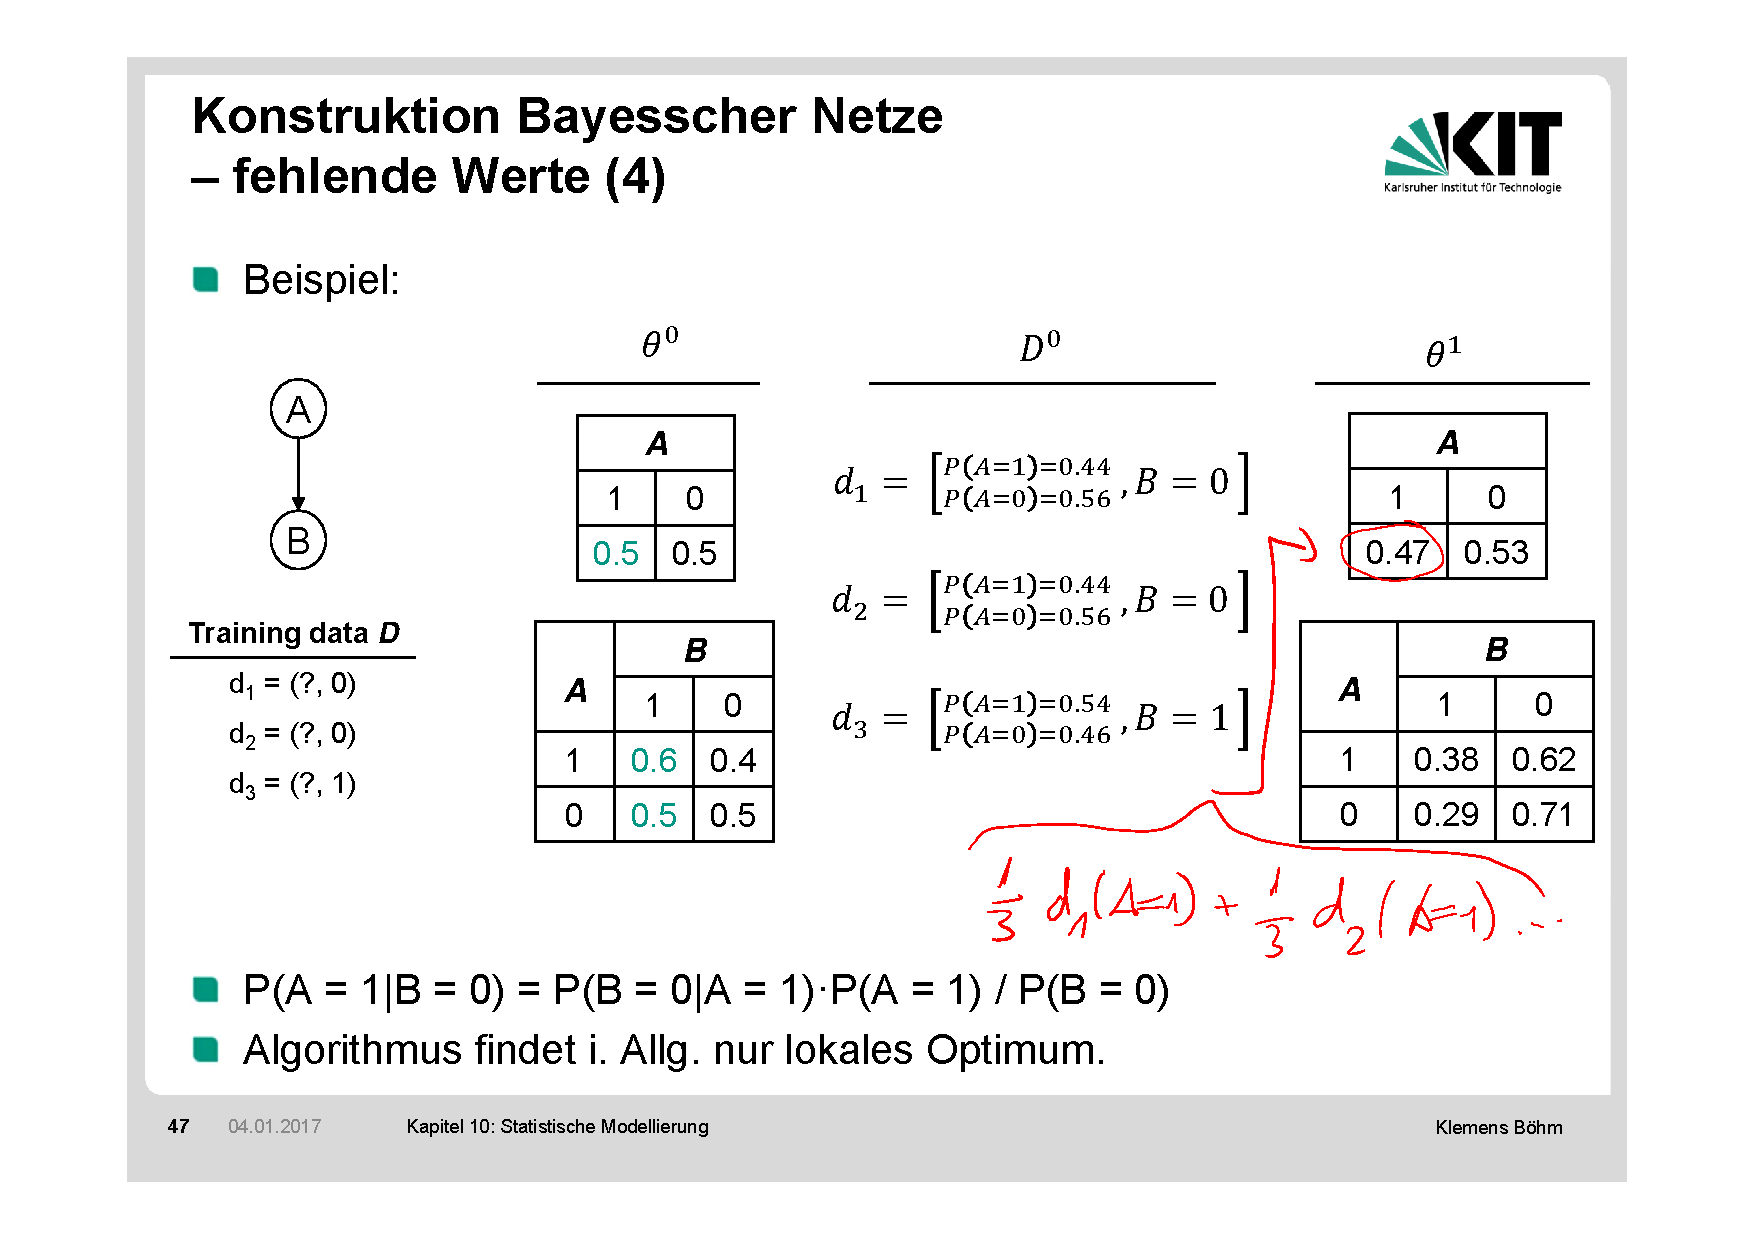
\includegraphics[width=0.75\textwidth]{Figures/BNEM}
	\caption[BN EM Beispiel]{Beispiel für ein Bayesian Network mit EM Lerner.\footnotemark}
	\label{fig:bnem}
\end{figure}
\footnotetext{11. Foliensatz, S.47, Analysetechniken für große Datenbestände, Prof. Dr.-Ing. Klemens Böhm}

Am besten wir hier das Vorgehen durch Abb.~\ref{fig:bnem} visualisiert.
Die grünen Werte in den Anfangstabellen werden geraten, wodurch sich die übrigen Werte bestimmen lassen. Sind die Tabellen ausgefüllt,
so werden die Wahrscheinlichkeiten für die jeweiligen 
Klassenzugehörigkeiten mit der dargestellten Formel berechnet; auch hier
gilt, dass man \(P[B]\) nicht berechnen muss, da es durch Normalisieren
im nächsten Schritt entfällt. Damit lassen sich dann die anderen Werte
für die nächsten Schritte berechnen.

Ein letztes Verfahren wäre gradient descent gewesen, das in der Vorlesung
jedoch ausgelassen wurde.

\subsection{Anwendung Bayesian Networks: Duplikaterkennung}
Ein Anwendungsgebiet von Baysian Networks ist die Duplikaterkennung.
Daten können durch menschliche Fehler in unserem Datenbestand
doppelt vorkommen, jeweils mit kleinen Unterschieden. Dies ist ein
Spezialfall von Klassifikation, nämlich ob ein Paar von Datensätzen ein
Duplikat ist, oder nicht. 

Dies ist auch schon die Transformation für unsere Daten: Wir 
betrachten die Daten nämlich nun im Folgenden nicht mehr
einzeln, sondern Paarweise und unsere Klassen sind nun 
Duplikat: ja oder nein.

Betrachten wir ein einzelnes Attribut: Es gibt zig mögliche Varianten,
wie man die Ähnlichkeit zwischen zwei Ausprägungen des Attributs
messen kann. Erweitert man dies nun auch noch um die Abhängigkeiten
zwischen den einzelnen Attributen, so hat man ganz schnell ein 
unhaltbar komplexes Netzwerk. Insbesondere wird es dann komplex,
wenn wir kontinuierliche Ähnlichkeitsmaße haben. Die Grenzen zwischen
ja und nein für unsere Duplikaterkennung verwischen immer mehr.

Deswegen kann mit sich mithilfe von \textbf{Hidden Variables} das
Leben deutlich erleichtern. Diese sind binäre Variablen, die zwischen
die Abhängigkeiten geschaltet werden und lediglich angeben,
ob ein Paar fast übereinstimmt oder gar nicht ähnlich ist. Sie stellen eine
Abstraktion vom Kontinuierlichen in das Binäre dar, während die
Abhängigkeiten zwischen den Attributen in gewisser Weise erhalten
bleiben (nicht in der Qualität, wie ohne diese Hidden Variables, aber
immerhin lässt sich das Problem jetzt noch berechnen).